\section{Tecnologie utilizzate}
Le tecnologie impiegate per il progetto in questione sono state tra le prime cose dibattute e definite, previa fase di modellazione dell'applicativo. Ogni tecnologia, framework e ambiente di sviluppo è stato scelto valutando la fattibilità, la coerenza e l'impiego ottimale di risorse oltre che all'ottimizzazione delle prestazioni. In questa prima fase ci siamo soffermati affinché potessimo garantire che ogni tecnologia utilizzata potesse permetterci di costruire un solido sistema distribuito, che pertanto avesse tutte le caratteristiche fondamentali di esso. In seguito andremo ad indicare e descrivere le principali tecnologie utilizzate suddividendole in server side, client side e database.

\subsection{Server-side}
Per quanto riguarda il lato server la nostra scelta è ricaduta sull'utilizzo di Java e sull'ausilio di Gradle. Abbiamo adottato un'architettura a microservizi utilizzando Vert.x il chè ci ha permesso di distinguerci dagli approcci monolitici tradizionali suddividendo le funzionalità cardine dell'applicazione. Tale approccio inoltre supporta la scalabilità dinamica ed agevola l'integrazione di nuove caratteristiche, oltre a suddividere funzionalità di base permettendo anche un più agile sviluppo suddividendo il carico di lavoro tra diversi programmatori. Ciascun servizio è idealmente indipendente e non influisce sugli altri servizi nell'infrastruttura, di conseguenza, l'eventuale errore di un componente non determina il blocco dell'intero applicativo, come avverrebbe con altre architetture di natura monolitica. Di seguito analizzeremo le principali tecnologie utilizzate lato server, sottolineandone le peculiarità che ci hanno spinto ad impiegarle nel progetto.
\label{sub:server-tech}

\subsubsection{Gradle}

Gradle è un Tool per il Building di
applicativi Java che permette di scaricare dipendenze, compilare e testare il codice con uno sforzo minimo.\newline

\noindent L'interfaccia da riga di comando è uno dei metodi principali per interagire con Gradle.
L'uso del Gradle Wrapper è fortemente incoraggiato. Sarebbe opportuno sempre sostituire ./gradlew o gradlew.bat con gradle qualora si usasse un wrapper.

\noindent L'esecuzione di Gradle da riga di comando è conforme alla seguente struttura. Le opzioni sono consentite prima e dopo i nomi delle attività.

\begin{minted}{bash}
    $ gradle [taskName...] [--option-name...]
\end{minted}

\noindent È possibile inizializzare un'aplicazione Java tramite il seguente comando:
\begin{minted}{bash}
    $ gradle init --type java-application
\end{minted}

\noindent Le dipendenze potranno poi essere aggiunte nel file generato \textit{build.gradle}.\newline

Per la creazione del Web-Server verrà utilizzata  Vert.X, una libreria che verrà illustrata nella prossima sezione.\newline
Vert.X mette a disposizione molteplici dipendenze importabili tramite Gradle.
Per importare gli elementi core di Vert.X nella sezione dependencies deve essere aggiunta la seguente stringa:
\begin{minted}{java}
val vertxVersion = "3.9.4"
dependencies {
      implementation("io.vertx:vertx-core:$vertxVersion")
}
\end{minted}

\noindent Vert.X offre tuttavia anche un template Gradle di un Web-Server d'esempio in cui sono già importate le dipendenze di base ~\cite{vertx3ve91:online}.
La base del progetto finale sarà questo template, a cui verranno aggiunte altre dipendenze, come package di Vert.X secondari o librerie per gestire la connessione con il Database o la generazione di PDF.

\noindent Gradle offre anche molteplici funzionalità per gestire la build del progetto o addirittura il deploy.

\noindent Eseguendo il seguente comando, dopo aver opportunamente modificato i file di configurazione, l'applicazione viene eseguita.
\begin{minted}{java}
    $ gradle run
\end{minted}

\noindent Eseguendo il seguente comando invece verranno eseguiti i test dell'applicazione:
\begin{minted}{java}
    $ gradle test
\end{minted}

Gradle offre anche la possibilità di creare Task personalizzati.
\begin{figure}[H]
    \caption{Logo di Gradle ~\cite{GradleEnterprise:online}}
    \centering
    
\includegraphics[width=100mm]{img/logos/gradle_logo.png}
    \label{fig:gradle_logo}
\end{figure}

\subsubsection{Vert.X}
Tramite la piattaforma VertX è possibile rilasciare ed eseguire le proprie applicazioni, sia lato client che lato server (nel nostro progetto abbiamo esplorato il lato server).\newline
Per alcuni aspetti, risulta simile a Node.JS ma con una differenza di spessore: viene eseguito tramite Java Virtual Machine, è scalabile, concorrente, non bloccante, distribuito e sviluppabile tramite molteplici linguaggi.\newline

\noindent Sviluppato originariamente con il nome di Node.x nel 2011, per evitare problemi legali legati alla similitudine con il nome "Node.js", il nome è stato cambiato in Vert.x, mantenendo lo stesso significato: "vertex" difatti è sinonimo di "nodo" in matematica.\newline
Le funzionalità del core occupano poco spazio sia in termini di codice che di memoria, rendendo il framework Vert.x molto leggero.
\begin{figure}[H]
    \caption{Logo di Vert.X ~\cite{VertX:online}}
    \centering
    
\includegraphics[width=100mm]{img/logos/vert_x_logo.png}
    \label{fig:vert_x_logo}
\end{figure}

\paragraph{Verticles}\mbox{}\\
Un applicativo Vert.x è composto da uno o più componenti denominati \emph{Verticle}.\newline
Ognuno dei Verticle componenti il sistema viene eseguito in maniera
concorrente ed autonoma rispetto agli altri; non è dunque presente uno stato condiviso tra di essi.\newline

\noindent Tramite il framework Verx.x dunque è possibile sviluppare applicazioni multi-threaded senza il bisogno di gestire problematiche quali la sincronizzazione tra i thread in esecuzione.

\paragraph{Event Bus}\mbox{}\\
Attraverso questo componente è possibile scambiare messaggi tra i vari Verticle che compongono il sistema.\newline

\noindent Una caratteristica fondamentale dell'eventbus è la sua predisposizione alla comunicazione nei sistemi distribuiti: attraverso di esso, infatti, è possibile collegare verticle in esecuzione su diverse JVM.\newline
Al fine di ottenere tale comunicazione in ambito distribuito è sufficiente registrarsi ad uno specifico indirizzo sull'Event Bus e creare un \emph{Event Handler}; tale handler verrà richiamato ogni qual volta che un nuovo evento (messaggio sull'Event Bus) sarà scatenato da uno dei Verticle connessi a tale indirizzo.

\paragraph{Eventi bloccanti}\mbox{}\\
Nel caso in cui un Verticle esegua un numero elevato di operazioni di input/output (le quali si protraggono a lungo nel tempo) la coda degli eventi rimane bloccata fino al termine di tali operazioni; questo è un problema in quanto nessun altro messaggio verrà instradato verso gli altri Verticle i quali non potranno dunque reagire in modo concorrente agli eventi.\newline

\noindent Vert.x propone come soluzione a questo problema un tipo particolare di Verticle, denominato \emph{Worker}, grazie alla quale le operazioni non risulteranno bloccanti.

\paragraph{Sviluppo multi-linguaggio}\mbox{}\\
Vert.x offre la possibilità di sviluppare i singoli componenti tramite diversi linguaggi.\newline

Nel nostro progetto sono stati utilizzati:
\begin{itemize}
    \item {\emph{Java}, per lo sviluppo dell'intero server}
    \item{\emph{JavaScript}, per la creazione di web-socket lato client in grado di comunicare con l'Event Bus di Vert.x (tramite il supporto della libreria SockJS, che verrà approfondita a breve)}
\end{itemize}

\subsubsection{gson}
gson è una libreria Java Open Source che può essere utilizzata per convertire oggetti Java nella loro rappresentazione JSON.\newline
Può anche essere utilizzata per convertire una stringa JSON in un oggetto Java equivalente
~\cite{gsonIniz52:online}.\newline

\noindent Vert.X offre già delle API per creare oggetti ed array in formato JSON in modo semplice e veloce grazie alle classi JsonObject ~\cite{JsonObj:online} e JsonArray ~\cite{JsonArr:online}.\newline

\noindent L'utilizzo di ulteriori librerie per la serializzazione e deserializzazione del formato JSON è tuttavia incoraggiato perché permette di rendere più semplici conversioni di oggetti più complessi e corposi, come le collezioni.

\noindent Gson offre una vasta gamma di operazioni possibili, tra le quali:

\begin{itemize}
\item Meccanismi semplici da usare come \textit{toString()} e metodi Factory per convertire oggetti Java in JSON e viceversa;

\item Conversione da e verso JSON di oggetti non modificabili preesistenti;

\item Supporto ad oggetti arbitrariamente complessi;
\item Generazione di output JSON compatto e leggibile.
\end{itemize}

\noindent Il codice sorgente di Gson è disponibile su Github ~\cite{googlegs79:online}.

\begin{figure}[H]
    \caption{Logo di gson ~\cite{googlegs79:online}}
    \centering
    
\includegraphics[width=100mm]{img/logos/gson_logo.png}
    \label{fig:gson_logo}
\end{figure}

\subsection{Client-side}
Per il lato client è stato scelto uno stack tecnologico che ci permettesse il più possibile il riutilizzo di codice e l'automazione.\newline
È stato dunque scelto l'utilizzo di javascript con l'appoggio di node.js grazie ai quali è stato possibile realizzare agilmente sia la versione web del client che quella mobile nativa.\newline
\label{sub:client-tech}
\subsubsection{Node Package Manager}

\noindent Node.js ~\cite{nodejs:online} è una runtime di JavaScript multipiattaforma per l'esecuzione di codice JavaScript, costruita sul motore JavaScript V8 di Google Chrome.\newline
Node.js dispone di una grande quantità di moduli scritti completamente in Javascript.
Essendo il progetto open source è inoltre possibile per gli sviluppatori aggiungere i propri moduli in modo da renderli disponibili pubblicamente ~\cite{nodejs:online}.\newline
\noindent Il gestore di pacchetti predefinito per l'ambiente di runtime JavaScript Node.js si chiama Node Package Manager (npm).
npm può essere richiamato tramite linea di comando usando la seguente sintassi:
\begin{verbatim}
    npm <command> [args]
\end{verbatim}
Il comando base per ottenere un pacchetto è:
\begin{verbatim}
    npm install packet_name
\end{verbatim}
Tutte le dipendenze e i conflitti vengono gestiti automaticamente ~\cite{npmDo:online}.
\newline Grazie a Node.js è possibile creare un progetto React utilizzando il comando seguente:
\begin{verbatim}
    npx create-react-app project
\end{verbatim}
\textbf{npx} è uno strumento integrato in npm in grado di eseguire pacchetti, anche se non sono ancora installati nel sistema.\newline
Sarà poi possibile avviare il server di sviluppo usando i seguenti comandi:
\begin{verbatim}
    cd project
    npm start
\end{verbatim}
L'interfaccia sarà poi visualizzabile all'indirizzo \texttt{http://localhost:3000} ~\cite{PrimiPas97:online}.

\begin{figure}[H]
    \caption{Logo di npm ~\cite{npm:online}}
    \centering
    
\includegraphics[width=40mm]{img/logos/npm_logo.png}
    \label{fig:npm_logo}
\end{figure}

\subsubsection{React.js}
React è un framework open-source che permette di implementare applicazioni web seguendo i principi della
programmazione ad oggetti. In modo particolare risulta essenziale comprendere tre
concetti chiave:
\begin{itemize}
    \item \textbf{JSX}\\
    JSX ~\cite{introduzione_jsx_react} è un'estensione della sintassi di JavaScript.\newline
    Permette di unire gli aspetti di html come linguaggio di template agli aspetti di JavaScript come linguaggio di scripting in una forma che ne aumenta semplicità e leggibilità.\newline
    Gli elementi JSX vengono utilizzati nelle definizioni delle funzioni di rendering (che verranno trattate a breve) semplificando la costruzione della user interface.\newline
    Attraverso JSX possiamo richiamare un componente React tramite con un meccanismo analogo ai tag in html.
    \item  \textbf{Componenti}\\
    Attraverso un componente ~\cite{componente_react} andiamo a definire quella che risulta essere a tutti gli effetti una classe.\newline
    Il nostro componente, definito da uno o più costruttori, contiene uno stato; questo stato verrà mantenuto, ed eventualmente aggiornato, durante tutto il ciclo di vita (lifecycle) del componente.\newline
    È possibile ricevere dati ed istruzioni da altri componenti attraverso le props.\newline
    \item \textbf{Stato}\\
    Lo stato ~\cite{state_e_lifecycle_react} un insieme di proprietà di un componente.\newline
    Queste proprietà possono variare a seguito dell'interazione con altri componenti o come azione del componente stesso nel caso esso esegua delle azioni a cadenza temporale.\newline
    In React inoltre lo stato risulta fondamentale ai fini di ottenere un rendering a schermo performante; ogni componente React infatti deve obbligatoriamente definire una funzione \emph{render()}.\newline
    Attraverso di essa verrà ritornato il contenuto da renderizzare a schermo.\newline
    React cambierà il contenuto a schermo (consumando quindi risorse) solamente quando vi saranno delle modifiche nel contenuto ritornato dalla funzione render(); utilizzando dunque le proprietà che definiscono lo stato del componente all'interno della funzione render() del componente stesso riusciremo a ridurre al minimo indispensabile il numero di volte in cui l'applicazione verrà renderizzata, riflettendo i cambiamenti di stato del componente.
\end{itemize}
\begin{figure}[H]
    \caption{Logo di React.js ~\cite{React:online}}
    \centering
    
\includegraphics[width=40mm]{img/logos/react_logo.png}
    \label{fig:react_logo}
\end{figure}
\subsubsection{Redux}
Redux ~\cite{caratteristiche_redux} è un \emph{contenitore di stato} per applicazioni JavaScript.\newline
Gode di quattro caratteristiche fondamentali per progetti portata medio-grande:
\begin{itemize}
  \item \textbf{Deterministico}\\
  Un aspetto fondamentale nelle applicazioni web di ogni genere è il determinismo.\newline
  L'oneroso compito di far collaborare tutti i componenti al fine di ottenere un comportamento predicibile viene largamente semplificato dal framework Redux.
  \item \textbf{Centralizzato}\\
  Avere stato e logica centralizzati permette di ottenere rapidamente delle feature di fondamentale importanza, come funzioni di "annulla" e "ripeti" che ci permettono di muoverci agilmente tra lo storico degli stati.\newline
  Inoltre un approccio centralizzato garantisce un consistenza maggiore dei dati, rendendo possibile modificarli solamente attraverso specifiche funzioni (azioni) create durante la definizione della struttura dati.
  \item \textbf{Debug oriented}\\
  Attraverso semplici plugin browser come Redux DevTools risulta immediato il debug dell'applicazione.\newline
  Difatti attraverso questi tool otteniamo una visione completa dello stato dei dati e della sua evoluzione nel tempo, riuscendo ad identificare con precisione quando e soprattutto perchè lo stato abbia subito delle modifiche.
  \item \textbf{Flessibile}\\
  Redux funziona con ogni layer di User Interface e, essendo ormai uno strumento consolidato, dispone di un solido supporto e un vasto parco di plugin e pacchetti aggiuntivi per ogni esigenza.
\end{itemize}
Per comprendere come queste caratteristiche si concretizzino risulta fondamentale comprendere tre concetti chiave nella struttura di Redux:
\begin{itemize}
  \item \textbf{Store}\\
  Lo store ~\cite{store_redux} è un oggetto che contiene l'intera struttura ad albero dello stato.\newline
  Fornisce metodi per la lettura dello stato corrente.
  \item \textbf{Reducer}\\
  I reducer ~\cite{reducer_redux} definiscono la struttura dello store.\newline
  Vi possono essere più reducer all'interno di una stessa applicazione, al fine di meglio suddividere lo stato.
  \item \textbf{Azioni}\\
  Le azioni ~\cite{azioni_redux} permettono di modificare il contenuto dello store.\newline
  Essendo queste l'unico modo per alterare lo stato attuale, qualsiasi componente che voglia agire sullo stato deve passare per le azioni definite.
\end{itemize}
Ma \emph{perchè} utilizzare un contenitore di stato se ogni componente React possiede già uno stato?
React, pur essendo uno strumento molto potente, ci pone davanti a delle limitazioni:
\begin{itemize}
  \item
  Innanzitutto non è raro che più componenti debbano fare riferimento allo stesso dato; la presenza di uno stato comune evita di dover implementare meccanismi ad hoc di sincronia tra gli stati dei due componenti.\newline
  Lo stato di ogni componente, attraverso tool ready to use, sarà dunque sincronizzato con la struttura principale.
  \item
  In secondo luogo React incoraggia lo scambio di dati solo in una direzione: da un componente padre verso un componente figlio (utilizzato dunque dal padre).\newline
  La presenza delle azioni Redux risolvono questo problema in quanto ogni cambiamento apportato allo stato Redux si rifletterà su tutti i componenti React che utilizzano quel particolare dato.
\end{itemize}
\begin{figure}[H]
    \caption{Logo di Redux ~\cite{redux:online}}
    \centering
    
\includegraphics[width=70mm]{img/logos/redux_logo.png}
    \label{fig:redux_logo}
\end{figure}

\subsubsection{SockJS}
\noindent SockJS è una libreria JavaScript che fornisce un servizio molto simile alle originali Web-Socket. SockJS offre delle API JavaScript cross-browser che permettono la creazione di un canale di comunicazione full-duplex tra domini a bassa latenza tra il browser e il server web. \newline

\noindent SockJS tenta di utilizzare prima di tutto le WebSocket native. In caso fallisca (in caso di incompatibilità coi sistemi o a causa di altri problemi)
ricorrerà all'utilizzo di una varietà di protocolli di trasporto specifici del browser astraendoli in modo simile al funzionamento di una WebSocket. \newline

\noindent SockJS è stato progettato per funzionare con tutti i browser moderni e in ambienti che non
supportano il protocollo WebSocket, ad esempio dietro proxy aziendali restrittivi. ~\cite{GitHubso32:online} \newline

\noindent Sul repository ufficiale di SockJs è riportata la filosofia su cui si basa, riassunta nei seguenti punti:
\begin{itemize}
    \item le API dovrebbero attenersi per quanto possibile alle WebSocket API di HTML5;
    \item tutti i trasporti devono supportare connessioni interdominio predefinite;
    \item esiste ed è garantito il supporto per almeno un protocollo di streaming per ogni browser principale;
    \item i trasporti in streaming dovrebbero dovrebbero supportare i cookie e funzionare su più domini;
    \item il polling viene impiegato come fallback per vecchi browser e host dietro proxy restrittivi;
    \item la connessione dovrebbe sempre essere stabilita in modo veloce e leggero.
\end{itemize}


\begin{figure}[H]
    \caption{Logo di SockJS ~\cite{sockjsso96:online}}
    \centering
    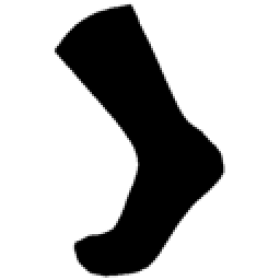
\includegraphics[width=35mm]{img/logos/sockjs_logo.png}
    \label{fig:sockjs_logo}
\end{figure}

\subsubsection{React Native}
React Native è un framework open-source che permette lo sviluppo nativo mobile tramite l'utilizzo di JavaScript e JSX.\newline
Il punto di forza di tale framework è la possibilità di ottenere un vero "write once, run everywhere", minimizzando i tempi di sviluppo; React Native infatti può essere utilizzato per lo sviluppo su entrambe le piattaforme mobile più diffuse sul mercato: Android e iOS.\newline
React Native inoltre (anche se questo aspetto non è stato affrontato nell'ambito di questo progetto) permette di sviluppare per Android TV, macOS, tvOS, Windows e UWP.\newline
A livello implementativo React Native utilizza, quasi nella totalità, gli stessi costrutti della controparte web prima citata.\newline
Se React per il web per funzionare agisce manipolando il DOM, React Native agisce in un processo in background all'interno del client mobile; in tale processo il codice javascript viene interpretato, così che sia possibile interpretarlo nativamente nel dispositivo mobile.
\begin{figure}[H]
    \caption{Logo di React Native ~\cite{ReactNat38:online}}
    \centering
    
\includegraphics[width=35mm]{img/logos/react_native_logo.png}
    \label{fig:react_native_logo}
\end{figure}

\subsection{Database-side}
Un DBMS è un servizio software, realizzato come server in esecuzione continua, che gestisce uno o più database. I servizi che dovranno interagire con una base di dati non potranno manipolare ed accedere direttamente a questi ultimi, ma dovranno dialogare con il DBMS che sarà l'unico ad accedere fisicamente alle informazioni. Quanto detto implica che il DBMS sia il componente che si occupa di tutte le politiche di accesso, gestione, sicurezza ed ottimizzazione dei database. La nostra scelta per questo progetto è ricaduta su MySql, in quando perfettamente adatto alle nostre esigenze. Di seguito analizzeremo le sue principali caratteristiche.
\label{sub:db-tech}
\subsubsection{MySql}
MySql è un Database management system relazionale (RDBMS), tra le sue caratteristiche principali ritroviamo che esso è open source e libero. Al giorno d'oggi rappresenta una delle tecnologie più note e diffuse in ambito Database e nel mondo dell'IT in generale, e si uniforma allo standard più diffuso che è quello dei database relazionali, cioè appunto basati sulla teoria relazionale. Nasce nel 1996 come progetto dell'azienda svedese Tex, esso venne distribuito in modalità open source per favorirne la crescita. Negli ultimi 20 anni MySql si è diffuso molto velocemente prestando le sue caratteristiche e qualità a moltissimi software e siti. \newline

\noindent Il linguaggio SQL (Structured Query Language) è il formalismo che permette di indicare al DBMS quali operazioni svolgere sui database che gestisce. Tramite SQL si può infatti impartire qualsiasi tipo di operazione, sia sui dati che sulla struttura interna del database, sebbene le principali operazioni siano delle seguenti tipologie: inserimento, lettura, modifica e
cancellazione di dati, tipicamente indicate con l'acronimo CRUD (Create-Read-Update-Delete). \newline

\noindent Le caratteristiche principali di questo RDBMS sono:
\begin{itemize}
    \item ampia capacità di integrazione con i principali linguaggi di programmazione e ambienti di sviluppo più in generale;
    \item offerta di tutte le funzionalità tipiche dei migliori DBMS;
    \item ottima efficienza a prescindere dalla mole di dati che gli vengono affidate.
\end{itemize}

\begin{figure}[H]
    \caption{Logo di MySql ~\cite{redux:online}}
    \centering
    
\includegraphics[width=80mm]{img/logos/mysql_logo.png}
    \label{fig:mysql_logo}
\end{figure}
\newpage
